\section{结果}
\label{sec:results}

本节先报告三城市应用结论，再展开解释该结论所需的有限样本与实验特异证据。
表~\ref{tab:results_evidence_map} 概括每一层回答的问题及其解释边界。尤其需要
区分：正的 CMI 点估计在与估计量和设计相匹配的参考分布比较之前仍属描述性结果；
较低的 DELB 估计也不等同于较低的留出预测误差。

\begin{table}[H]
\begin{adjustwidth}{-\extralength}{0cm}
\caption{经验结果的证据解释图谱。}
\label{tab:results_evidence_map}
\scriptsize
\begin{tabularx}{\fulllength}{p{0.14\fulllength}XXX}
\toprule
\textbf{证据层} & \textbf{回答的问题} & \textbf{主要结果} & \textbf{解释边界} \\
\midrule
城市与局部点估计 &
加入自行车状态后，预测底线估计是否下降？ &
三个城市及所报告局部汇总的条件熵和相应 DELB 估计均下降。 &
描述经验状态划分差异，不能建立自行车特异信息。 \\
已知真值模拟与支持度诊断 &
总体 CMI 为零时，估计 CMI 是否仍可能为正？ &
稀疏嵌套状态产生正的 plugin 和 Miller--Madow 估计及非零随机化中心；
支持复杂度与两种现象均相关。 &
诊断有限样本估计与校准问题，不能证明城市层面的移动信息效应。 \\
随机化与多尺度校准 &
观测统计量相对于预设零机制是否异常大？ &
主要及多尺度比较均未通过相应校准和多重比较校正。 &
限制对近期、地理匹配自行车移动的归因，但不证明条件独立。 \\
匹配预测与 Predictability Gap &
拟合模型是否把增强状态转化为更低的留出 MSE？ &
改善依赖模型和城市，且只有两个纽约模型缩小估计 gap。 &
实际模型性能既不能证明也不能否定总体 DELB 的变化。 \\
Fano 对照 &
分类损失下是否保持相同的信息排序？ &
估计 Fano 底线下降，但稀疏条件下的留出众数分类器经常变差。 &
Fano 与 DELB 使用不同目标和损失，其数值不可直接比较。 \\
异质性与稳健性 &
描述性模式是否依赖目标或设定？ &
DELB 降幅点估计普遍为正，预测改善仍具有异质性。 &
目标和单位变化时不能直接比较效应量；分类结果属于探索性分析。 \\
\bottomrule
\end{tabularx}
\end{adjustwidth}
\end{table}

\subsection{三城市应用结果总览}
\label{subsec:application_results_overview}

\begin{table}[!htbp]
\caption{三个城市的应用层综合结果。E10 列为三种变换参考中最小的未修正
\(p\) 值；E18 列为基准状态匹配受限随机化的 \(p\) 值。正预测筛查在匹配的
城市--模型比较中完成校正。}
\label{tab:application_results_overview}
\centering
\footnotesize
\resizebox{\textwidth}{!}{%
\begin{tabular}{lrrrrrr}
\toprule
\textbf{城市} & \textbf{自行车域 \(\Delta L\)} &
\textbf{相对降幅} & \textbf{完整域 \(\Delta L\)} &
\textbf{E10 最小 \(p\)} & \textbf{E18 \(p\)} &
\textbf{正预测筛查 / gap 缩小}\\
\midrule
华盛顿特区 & 0.0123 & 7.9\% & 0.0119 & 0.967 & 0.599 & 0/4 \quad / \quad 0/4\\
纽约 & 0.0604 & 17.3\% & 0.0094 & 0.986 & 0.999 & 2/4 \quad / \quad 2/4\\
温哥华 & 0.0919 & 18.0\% & 0.0115 & 0.903 & 0.994 & 1/4 \quad / \quad 0/4\\
\bottomrule
\end{tabular}
}
\end{table}


应用结果呈现一致的描述性排序，但没有一致的推断或预测增益
（表~\ref{tab:application_results_overview}）。在自行车覆盖总体中，
加入滞后自行车流量后，华盛顿特区、纽约和温哥华的 DELB 估计分别下降
7.9\%、17.3\% 和 18.0\%。完整犯罪支持总体中的降幅仍为正，但纽约和
温哥华明显衰减。

E10 的三种变换参考和 E18 的基准状态匹配参考均未在任何城市分离出观测 CMI。
留出预测同样具有选择性：四类模型中，纽约有两类、温哥华有一类通过调整后的
正改善筛查，但只有纽约的两类模型缩小 Predictability Gap。因此，直接应用结论
不是“自行车移动一致改善犯罪预测”，而是：正的预测底线变化估计可以与校准参考
下的不拒绝及模型依赖的实际性能同时出现。以下各节展开这一综合结论背后的有限
样本和实验特异证据。

\subsection{CMI 估计的有限样本行为}
\label{subsec:results_e12_simulation}

该分析在解释任何城市结果之前隔离估计问题，目的是检验：在已知总体零假设下，
估计量本身是否会报告表观新增信息。在表~\ref{tab:e12_simulation_summary} 和
图~\ref{fig:e12_sparse_simulation} 中，估计量偏差是估计值与精确枚举总体 CMI
之差；随机化中心则是按指定机制变换数据后统计量的均值。二者均属于有限样本量，
但不能互相替代。

在解释城市点估计之前，已知总体真值的模拟首先回答 RQ2。即使总体 CMI
严格为零，估计 CMI 仍可能为正。在 72 个总体零假设设计单元中，plugin
估计的平均偏差为 \SimPluginNullBias{} bit，Miller--Madow 估计的平均偏差为
\SimMMNullBias{} bit。校正降低了平均偏差，但在最稀疏的设计中并未一致优于
plugin 估计。样本量从 365 增至 1095 时，两种估计量的平均零假设偏差均下降；
状态空间、singleton 占用率和有效自由度增加时，偏差上升。

变换特异的零分布中心同样为正：plugin 为 \SimPluginNullCenter{} bit，
Miller--Madow 为 \SimMMNullCenter{} bit。平均第一类错误率仍分别为
\SimPluginTypeI{} 和 \SimMMTypeI{}，因为推断比较的是观测统计量与完整参考分布，
而不是与零比较。正 CMI 设计下的平均 power 分别为 \SimPluginPower{} 和
\SimMMPower{}。

\begin{table}[!htbp]
\caption{Finite-sample CMI simulation summary. Null bias and null centers are in bits. Size is the mean rejection rate under population CMI equal to zero; power averages the positive-CMI designs.}
\label{tab:e12_simulation_summary}
\centering
\begin{tabular*}{\textwidth}{@{\extracolsep{\fill}}lcccc@{}}
\toprule
\textbf{Estimator} & \textbf{Mean null bias} & \textbf{Mean null center} & \textbf{Size} & \textbf{Power}\\
\midrule
Plug-in & 0.1651 & 0.2069 & 0.014 & 0.337\\
Miller--Madow & 0.1264 & 0.1376 & 0.011 & 0.447\\
\bottomrule
\end{tabular*}
\end{table}


\begin{figure}[H]
\begin{adjustwidth}{-\extralength}{0cm}
\centering
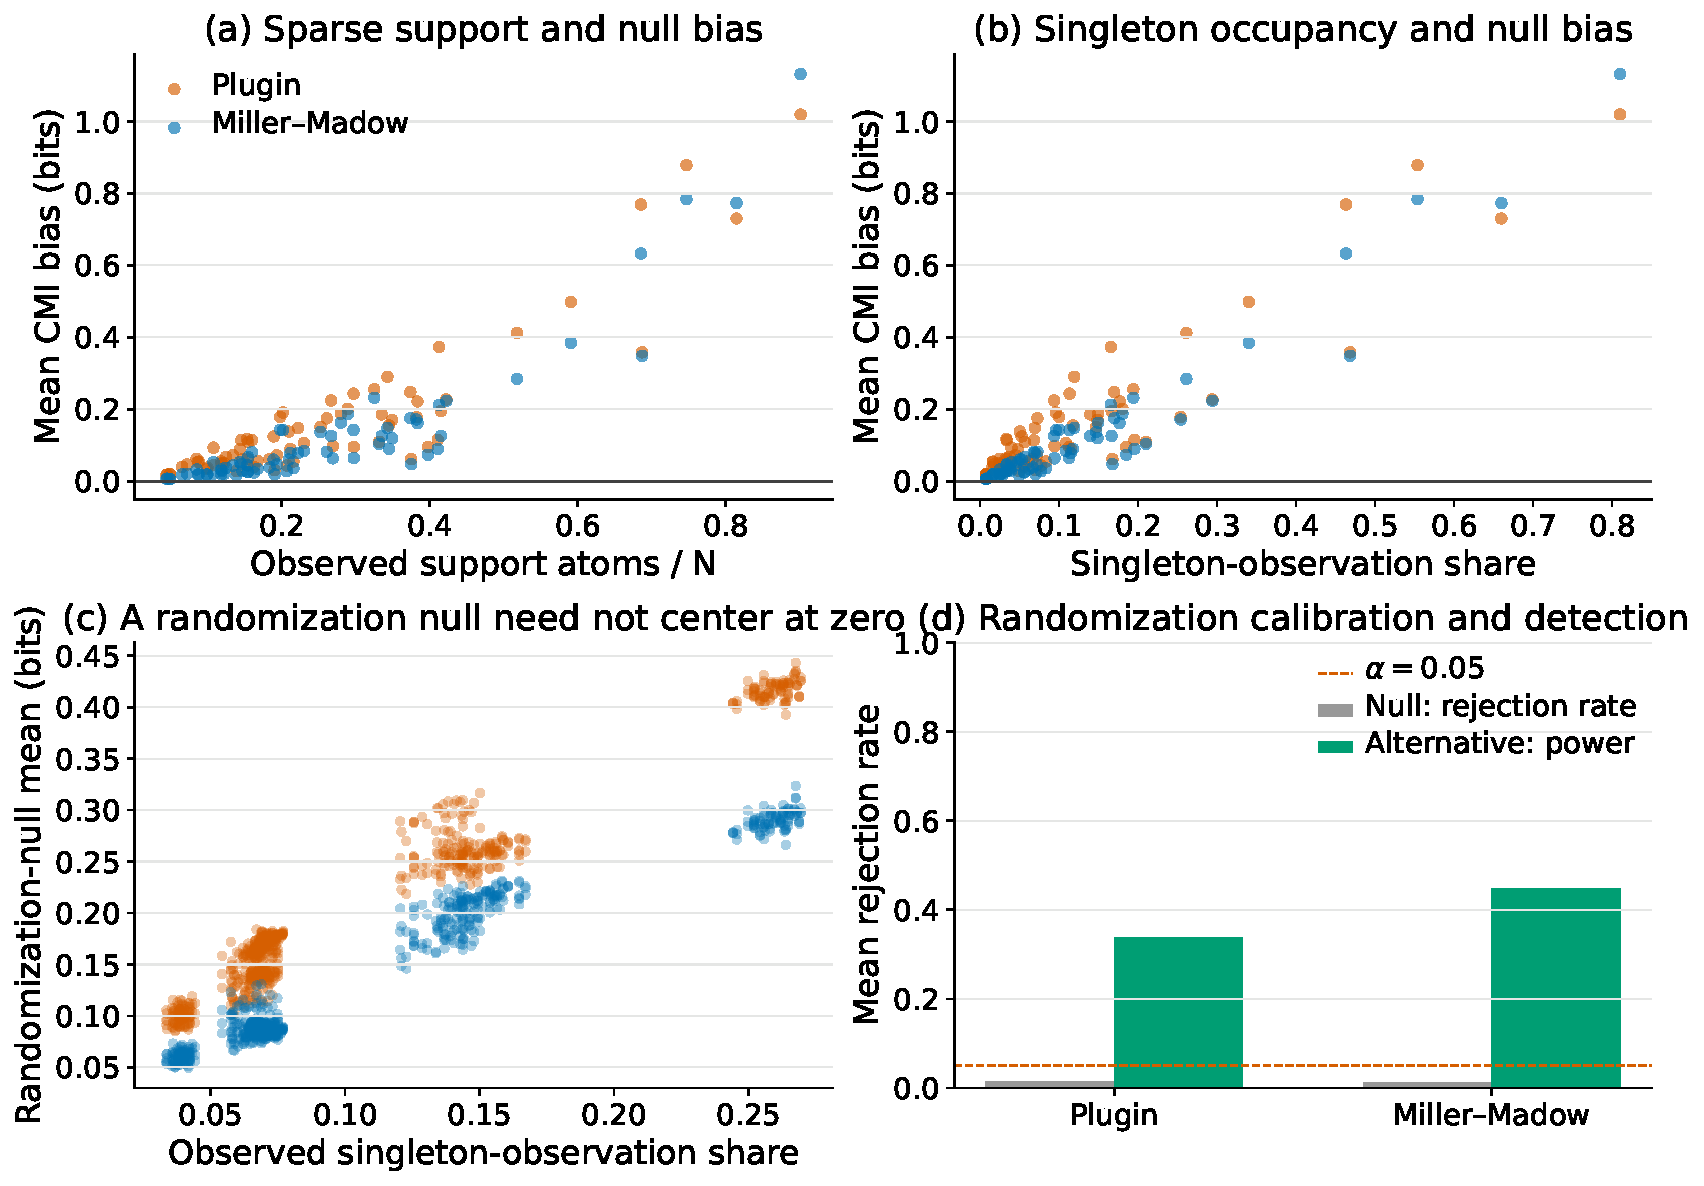
\includegraphics[width=\linewidth]{figures/s7/e12_sparse_cmi_main.pdf}
\end{adjustwidth}
\caption{稀疏嵌套状态下 CMI 估计与随机化行为的已知真值模拟。总体 CMI 由精确枚举
得到。正的估计量偏差与正的随机化中心是两个不同的有限样本对象。}
\label{fig:e12_sparse_simulation}
\end{figure}

因此，图~\ref{fig:e12_sparse_simulation} 的含义并不是正 CMI 必然虚假。
更准确地说，当新增变量把固定样本分割到大量低占用联合状态时，即使满足条件独立，
熵差也可能系统性上移。Miller--Madow 校正在这些设计中降低了平均偏移，但并未
消除使用设计匹配校准的必要性。

支持度诊断揭示了这一行为的机制。全部 8991 个城市替代统计量和 1,015,983 个
局部替代统计量均在冻结的 \(10^{-10}\)-bit 容差内复现，并在每次变换后重新计算
支持度。在已知零假设模拟中，观测原子密度、singleton 占用率和有效自由度与
plugin 及 Miller--Madow 偏差均强相关。在 1017 个城市--网格--零设计经验汇总中，
\(K_{\mathrm{obs}}/N\)、\(S_1\) 和 \(\nu/N\) 与零分布均值的相关系数分别为
0.835、0.866 和 0.988。

\begin{table}[H]
\caption{Association of support diagnostics with CMI estimator behavior. Entries are Spearman correlations. The first two columns use population-null simulations; the last two use 1,017 city-grid-null summaries.}
\label{tab:e13_support_relationships}
\begin{adjustwidth}{-\extralength}{0cm}
\centering
\small
\begin{tabular}{lrrrr}
\toprule
\textbf{Metric} & \textbf{Plugin bias} & \textbf{MM bias} & \textbf{Null mean} & \textbf{Observed--null}\\
\midrule
$K_{\mathrm{obs}}/N$ & 0.840 & 0.891 & 0.835 & -0.653\\
$S_1$ & 0.819 & 0.909 & 0.866 & -0.656\\
$\nu/N$ & 0.989 & 0.950 & 0.988 & -0.791\\
\bottomrule
\end{tabular}
\end{adjustwidth}
\end{table}


替代数据与观测数据之间的支持度变化同观测 CMI 减零分布均值负相关，相关系数范围为
\(-0.653\) 至 \(-0.791\)。在包含城市及零设计固定效应、并按城市--网格聚类
稳健标准误的模型中，替代 \(\nu/N\) 的系数为
\SupportCombinedNuCoefficient{}（SE \SupportCombinedNuSE{}），
\(R^2=\SupportCombinedNullRSquared{}\)。因此，支持结构解释了随机化中心的
大量变异，但这种关系既不是估计量偏差的恒等式，也不是因果关系。

\begin{figure}[H]
\begin{adjustwidth}{-\extralength}{0cm}
\centering
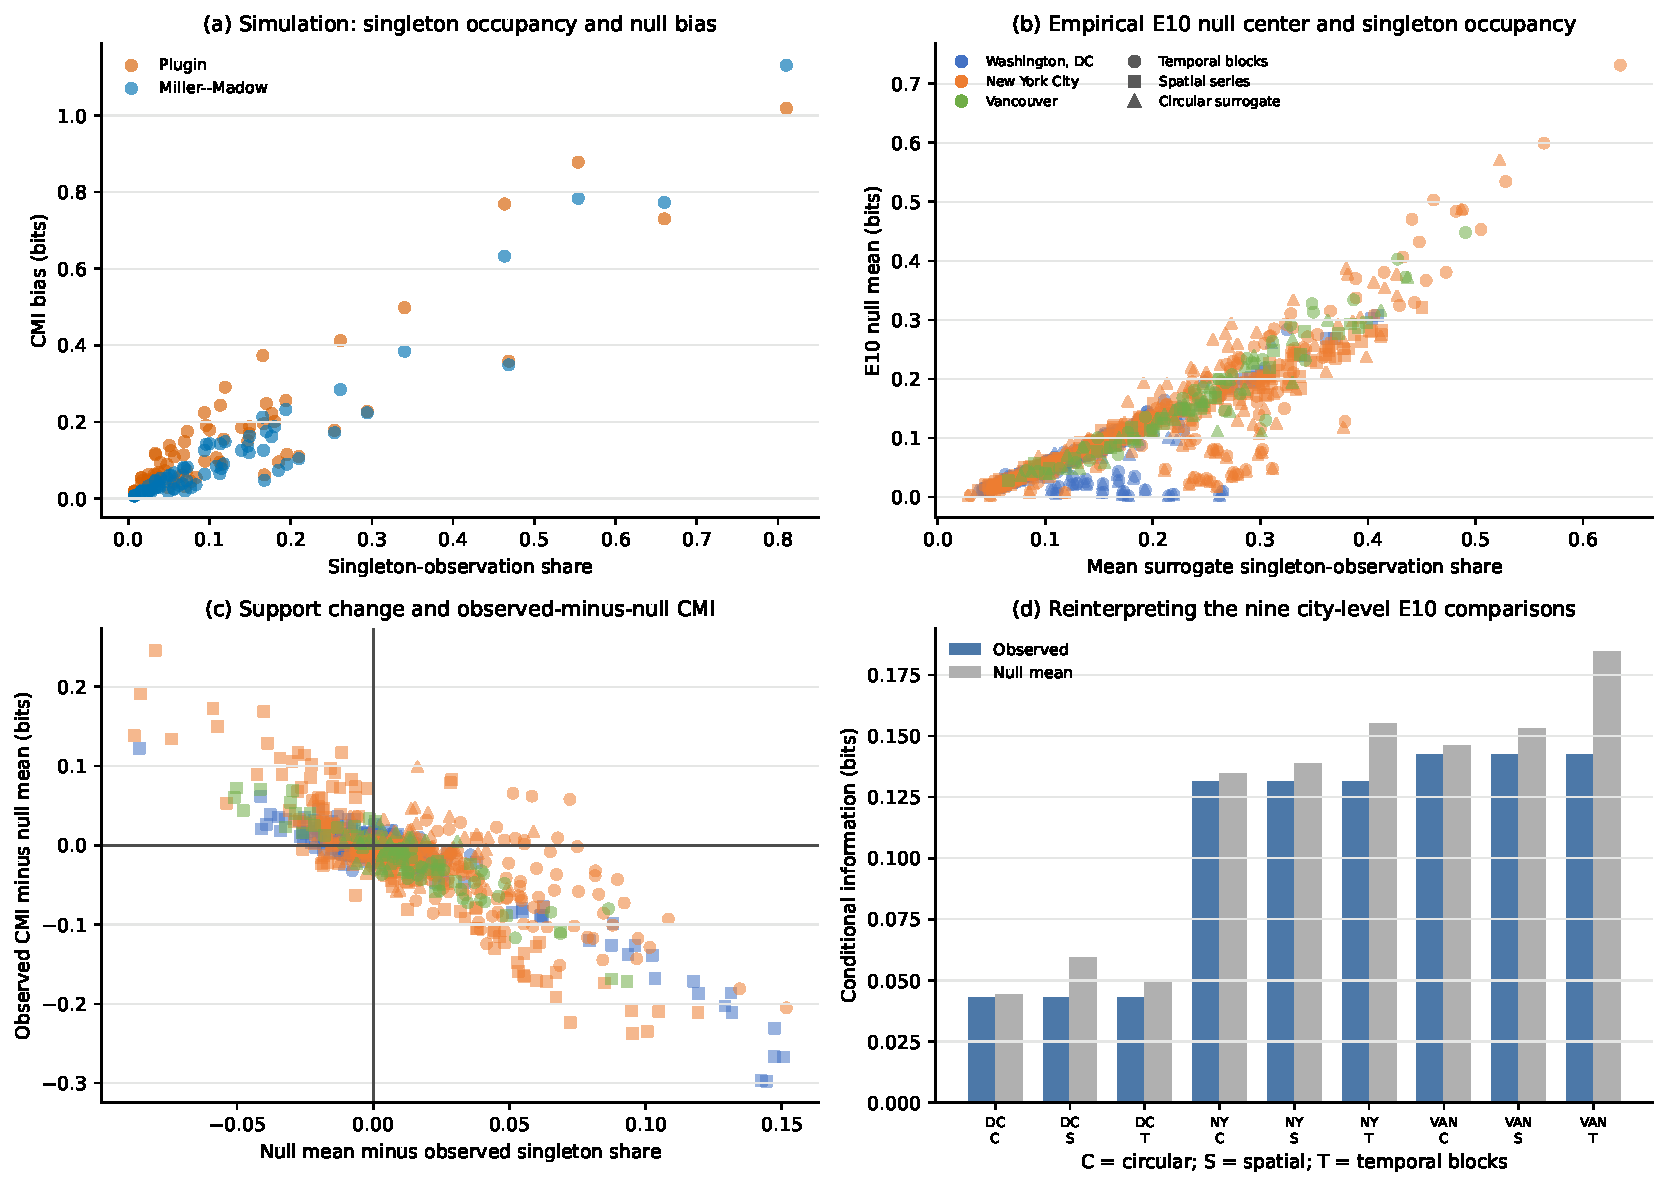
\includegraphics[width=\linewidth]{figures/s7/e13_support_null_main.pdf}
\end{adjustwidth}
\caption{支持结构与随机化零分布中心。模拟面板使用总体 CMI 已知为零的设计；
经验面板使用每次变换后重新计算的替代支持度。拟合线仅表示描述性关联。}
\label{fig:e13_support_null}
\end{figure}

图~\ref{fig:e13_support_null} 应被理解为参考分布中心的诊断：沿支持度轴移动表示
随机化改变了用于估计 CMI 的有效列联表。拟合关系不估计稀疏性的因果效应，也不能
据此减去一个通用偏差常数。模拟与支持度分析共同回答 RQ2 的估计部分：零不是合适的
自动有限样本基准；每次零机制变换后都必须重新计算统计量及其支持结构。

\subsection{城市与局部预测底线的点估计}
\label{subsec:results_city_information}

这一层回答描述性的总体导向问题：在加入离散化自行车状态后，估计不确定性及其隐含的
整数 MSE 底线下降多少？图~\ref{fig:city_information_bounds} 同时给出以 bit
表示的估计熵下降，以及把两个条件熵通过同一单调整数格最大熵包络逆映射后的
DELB 底线。

在上述有限样本限定下，表~\ref{tab:city_entropy_results} 报告主要城市汇总
点估计。加入滞后一天的自行车状态后，三个城市的条件熵估计均下降。
Miller--Madow CMI 在华盛顿特区、纽约和温哥华分别为 \DCCMI{}、\NYCMI{}
和 \VANCMI{} bit。经 \(\mathcal H_{\mathbb Z}^{-1}\) 映射后，对应的精确
DELB 降幅分别为 \DCDeltaL{}（\DCRelativeL）、\NYDeltaL{}
（\NYRelativeL）和 \VANDeltaL{}（\VANRelativeL）。


\begin{table}[H]
\caption{Pooled city-level conditional entropy and DELB results in the training bicycle-covered domain. Brackets report centered 95\% seven-day block-bootstrap intervals for CMI.}
\label{tab:city_entropy_results}
\begin{adjustwidth}{-\extralength}{0cm}
\centering
\begin{tabular*}{\linewidth}{@{\extracolsep{\fill}}lrrrrrrrr@{}}
\toprule
\textbf{City} & \(\boldsymbol{N}\) & \(\boldsymbol{H^0}\) &
\(\boldsymbol{H^B}\) & \textbf{CMI [95\% CI]} &
\(\boldsymbol{L^0}\) & \(\boldsymbol{L^B}\) &
\(\boldsymbol{\Delta L}\) & \(\boldsymbol{R^L}\)\\
\midrule
Washington, DC & 198,195 & 0.783 & 0.740 & 0.043 [0.040, 0.047] & 0.157 & 0.144 & 0.012 & 7.9\%\\
New York City & 216,810 & 1.293 & 1.162 & 0.131 [0.123, 0.140] & 0.350 & 0.290 & 0.060 & 17.3\%\\
Vancouver & 37,230 & 1.563 & 1.421 & 0.142 [0.126, 0.159] & 0.511 & 0.419 & 0.092 & 18.0\%\\
\bottomrule
\end{tabular*}
\end{adjustwidth}
\end{table}


\begin{figure}[!t]
\centering
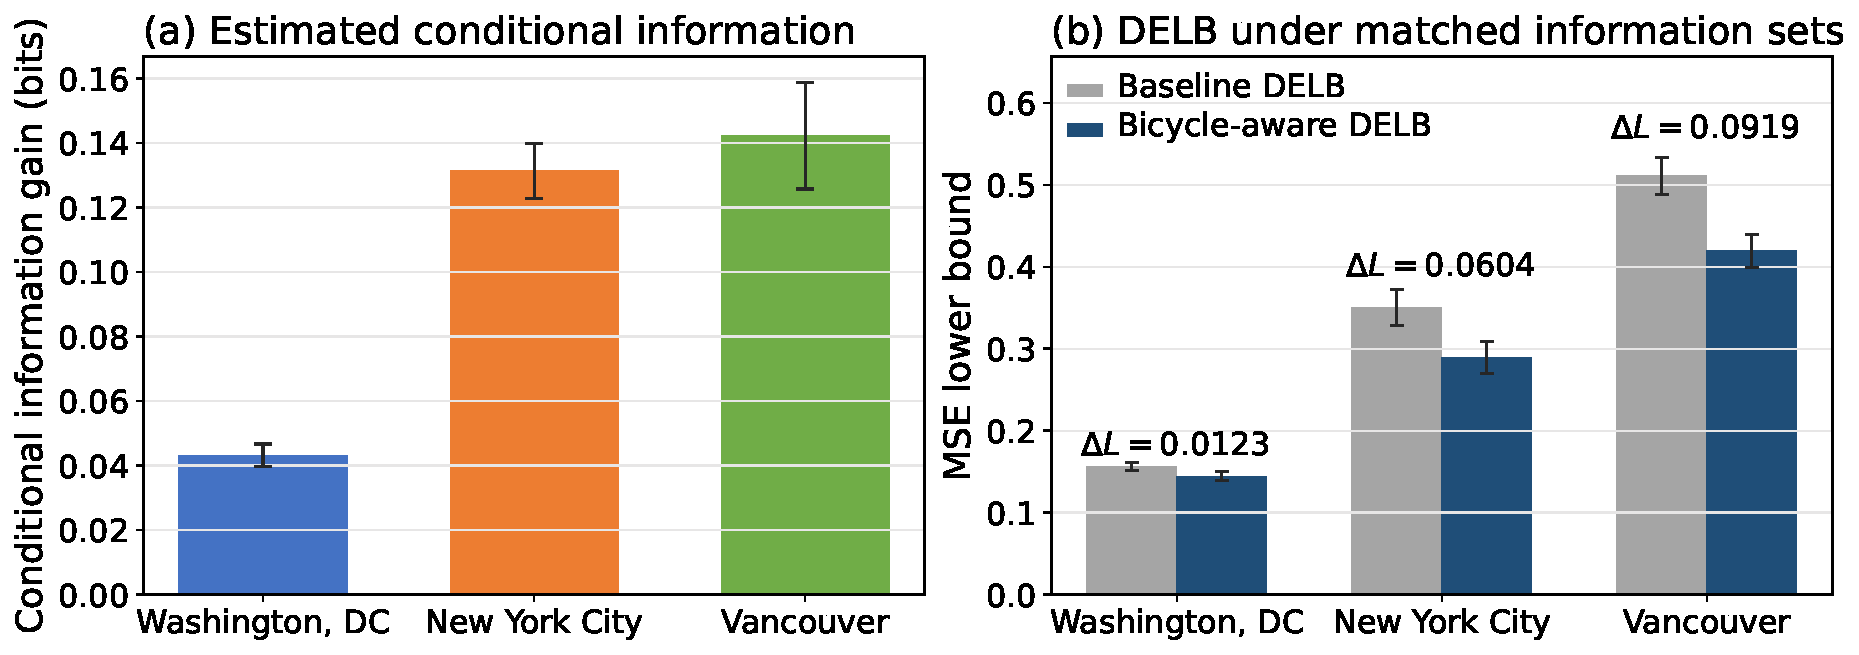
\includegraphics[width=\textwidth]{figures/e17/e17_city_cmi_delb_combined.pdf}
\caption{主要城市层面点估计。\textbf{(a)} Miller--Madow CMI 及中心化
95\% 七日区块 bootstrap 区间。\textbf{(b)} 基准与自行车增强信息集对应的
DELB 所隐含 MSE 底线。这些区间刻画观测支持度下的抽样波动；随机化校准见
第~\ref{subsec:results_nulls} 节。}
\label{fig:city_information_bounds}
\end{figure}
\FloatBarrier

\begin{table}[!htbp]
\caption{两个训练期冻结分析总体中的城市层面 DELB 点估计。完整犯罪支持域是
预先规定的完整目标总体；自行车覆盖域是其服务覆盖子集。}
\label{tab:co_primary_domains}
\centering
\footnotesize
\resizebox{\textwidth}{!}{%
\begin{tabular}{llrrrrrr}
\toprule
\textbf{城市} & \textbf{总体} & \textbf{网格} & \textbf{\(N\)} &
\textbf{CMI (bit)} & \textbf{\(L^0\)} & \textbf{\(L^B\)} &
\textbf{\(\Delta L\)}\\
\midrule
华盛顿特区 & 自行车覆盖 & 181 & 198,195 & 0.0432 & 0.1567 & 0.1443 & 0.0123\\
华盛顿特区 & 完整犯罪支持 & 186 & 203,670 & 0.0420 & 0.1535 & 0.1416 & 0.0119\\
纽约 & 自行车覆盖 & 198 & 216,810 & 0.1314 & 0.3503 & 0.2898 & 0.0604\\
纽约 & 完整犯罪支持 & 806 & 882,570 & 0.0348 & 0.1382 & 0.1288 & 0.0094\\
温哥华 & 自行车覆盖 & 34 & 37,230 & 0.1423 & 0.5113 & 0.4194 & 0.0919\\
温哥华 & 完整犯罪支持 & 141 & 154,395 & 0.0377 & 0.1774 & 0.1659 & 0.0115\\
\bottomrule
\end{tabular}
}
\end{table}


两个共同主要、训练期冻结总体中的城市层面点估计均为正
（表~\ref{tab:co_primary_domains}）。在完整犯罪支持域中，
华盛顿特区、纽约和温哥华的 CMI 分别为 0.0420、0.0348 和 0.0377 bit；在
自行车覆盖域中分别为 0.0432、0.1314 和 0.1423 bit。对应的完整域 DELB
降幅分别为 0.0119、0.0094 和 0.0115 MSE 单位，而服务域为 0.0123、
0.0604 和 0.0919。因此符号稳定，但纽约和温哥华的幅度明显依赖空间目标总体。
该共同主要比较仅适用于城市层面点估计；后续推断实验仍使用各自预先规定的
自行车覆盖总体。

因此，三个样本都呈现侧信息排序所需的第一阶段模式：增强后的经验状态对应较低的
预测底线估计。该结论针对观测到的状态划分。下降是否可特异归因于近期自行车移动，
是下文随机化结果回答的独立推断问题。

\subsubsection{局部点估计与空间格局}
\label{subsec:results_local_information}

局部分析关注预测底线估计的下降集中在哪里，而不是验证每个地图网格是否包含独立的
信息证据。完整表格与地图见补充材料 S2；颜色表示局部点估计的大小，不是显著性
尺度，Moran's \(I\) 则单独描述相近估计是否存在空间聚集。

413 个自行车覆盖网格中，共有 339 个满足局部分析条件：华盛顿特区 146 个、
纽约 160 个、温哥华 33 个。三个城市局部 \(\Delta L\) 中位数分别为
\DCLocalMedianDeltaL{}、\NYLocalMedianDeltaL{} 和 \VANLocalMedianDeltaL{}。
通过抽样不确定性筛查的网格分别为 137/146、155/160 和 33/33。

\(\Delta L\) 的全局 Moran's \(I\) 在华盛顿特区为 0.164
（\(p=0.002\)），纽约为 0.038（\(p=0.261\)），温哥华为 0.171
（\(p=0.022\)）。这些地图描述估计统计量的空间变异，并不能建立局部
自行车特异信息。

\subsection{随机化校准后的证据}
\label{subsec:results_nulls}

这是主要的归因层。此处问题不再是 CMI 是否为正，而是观测统计量相对于破坏预设时间
或空间对齐关系的数据变换是否异常大。在图~\ref{fig:city_nulls} 中，支持新增移动
信息需要观测标记位于相应参考分布的上尾；参考均值本身不必等于零。

随机化结果实质性限制了正点估计的解释。九个城市--设计比较均未拒绝其上尾参考：
\(p\) 值为 0.903--1.000，所有调整后 \(q\) 值均为 1.000。多数比较中，
观测 CMI 低于零分布均值。在局部尺度，339 个合格网格中同时通过三种设计的数量为
\LocalNullRejections{}，其中也包括已通过抽样不确定性筛查的网格。

E17 在三种熵估计器下得到相同的城市层面结论。每个估计器的九项比较中，
plugin 原始 \(p\) 值为 0.980--1.000，Miller--Madow 为 0.903--1.000，
Jeffreys--Dirichlet 为 0.984--1.000。估计器内部九项修正通过数为
\ESeventeenWithinRejects{}/27，全部 27 项全局修正通过数为
\ESeventeenGlobalRejects{}/27。完整估计器特定零分布汇总见补充材料 S1。


\begin{table}[H]
\caption{\rev{Randomization-reference calibration and distant-lag diagnostics.} Randomization
\(p\)-values are upper-tail tests of whether observed CMI exceeds the
specified null distribution. Distant-lag columns report
\(\widehat I_{\mathrm{distant}}/\widehat I_{\mathrm{recent}}\).}
\label{tab:null_calibration}
\centering
\begin{tabular*}{\linewidth}{@{\extracolsep{\fill}}lrrrrr@{}}
\toprule
\textbf{City} & \multicolumn{3}{c}{\textbf{Randomization \(p\)-value}} &
\multicolumn{2}{c}{\textbf{Distant/recent CMI}}\\
\cmidrule(lr){2-4}\cmidrule(lr){5-6}
 & \textbf{Temporal} & \textbf{Spatial} & \textbf{Circular} &
\textbf{14 days} & \textbf{30 days}\\
\midrule
Washington, DC & 1.000 & 1.000 & 0.967 & 0.992 & 0.985\\
New York City & 1.000 & 0.986 & 0.993 & 1.020 & 1.052\\
Vancouver & 1.000 & 0.969 & 0.903 & 0.964 & 1.007\\
\bottomrule
\end{tabular*}
\end{table}


\begin{figure}[!t]
\begin{adjustwidth}{-\extralength}{0cm}
\centering
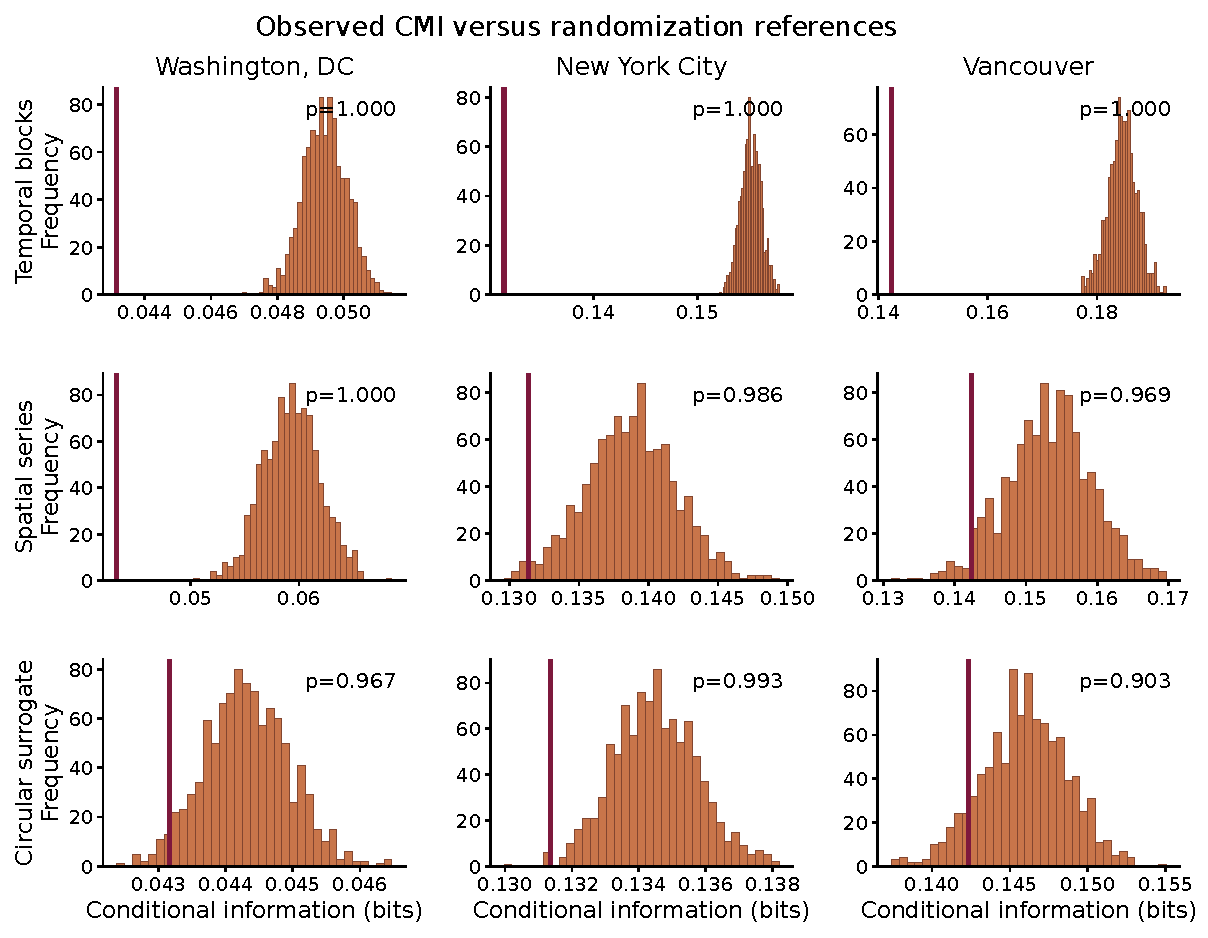
\includegraphics[width=\linewidth]{figures/e11/e10_city_null_distributions.pdf}
\end{adjustwidth}
\caption{城市层面观测 CMI 相对于时间区块、空间序列和循环移位参考分布的位置。
观测统计量未超过任何预设上尾参考。}
\label{fig:city_nulls}
\end{figure}

远期滞后给出相同解释。14 日或 30 日滞后 CMI 与匹配的一日滞后 CMI 之比为
\DistantRatioMin{}--\DistantRatioMax{}。在纽约，两个远期滞后均高于近期
滞后；在华盛顿特区和温哥华，差异较小且方向不一致。因此，这些诊断未能从统计量中
分离出近期且地理匹配的自行车信息。详细滞后图见补充材料 S2。

远期滞后比较提供了互补的特异性检查：若估计增益主要反映近期移动，一日状态应当与
明显更早的匹配状态分离。未观察到这种分离与缓慢共享时间结构的解释相符，但并不
构成对该机制的形式证明。

综合而言，对 RQ3 的回答是经校准且非因果的：点估计中存在表面信息增益，但无法将其
与所选随机化机制、稀疏支持度或缓慢的共享时间结构区分开。

\begin{table}[!htbp]
\caption{基准状态匹配的受限随机化及半合成校准。第一类错误率和功效来自拟合
离散度情景下每单元 50 个 Monte Carlo 数据集和每数据集 99 次随机化。}
\label{tab:e18_restricted_calibration}
\centering
\footnotesize
\resizebox{\textwidth}{!}{%
\begin{tabular}{lrrrrrrr}
\toprule
\textbf{城市} & \textbf{观测 CMI} & \textbf{零均值} &
\textbf{\(p\)} & \textbf{第一类错误率} &
\textbf{0.02 bit 功效} & \textbf{0.05 bit 功效} &
\textbf{最高评价 CMI 功效}\\
\midrule
华盛顿特区 & 0.0432 & 0.0433 & 0.599 & 0.04 & 0.10 & 0.06 &
0.0649 bit 时 0.48\\
纽约 & 0.1314 & 0.1338 & 0.999 & 0.08 & 0.02 & 0.02 &
0.1000 bit 时 0.46\\
温哥华 & 0.1423 & 0.1476 & 0.994 & 0.00 & 0.02 & 0.02 &
0.1000 bit 时 0.30\\
\bottomrule
\end{tabular}
}
\end{table}


基准状态匹配的受限随机化在三个城市的可移动块比例均为 1.00，并严格保持自行车
状态边际。其参考均值仍略高于观测 CMI（表~\ref{tab:e18_restricted_calibration}）。
华盛顿特区、纽约和温哥华的上尾 \(p\) 值分别为 0.599、0.999 和 0.994，
三项 BH 修正后 \(q\) 值均为 0.999。因此，使参考更接近基准状态并未改变
E10 的不拒绝结果。

半合成结果同时限制了这一解释。总体 CMI 为零时，受限设计在各城市和离散度
情景中的拒绝率为 0.00--0.08，所有精确二项式 95\% 区间均覆盖 0.05。
但在 0.02 和 0.05 bit 下，功效仅为 0.00--0.10。即使在拟合离散度情景中，
最高实际可达 CMI 下的功效在华盛顿特区、纽约和温哥华也仅为 0.48、0.46
和 0.30。固定经验支持下无法达到的高 CMI 情景按实际最大值报告。因此，
E18 支持受限参考的零校准，但也显示检测功效有限；其不拒绝不能证明条件无关。

\subsection{时空尺度与样本量校准}
\label{subsec:e16_scale_results}

该分析区分三个容易混淆的问题：改变空间或时间聚合会改变预测目标；保留不同比例的
时间块衡量固定设计下的估计稳定性；随机化则检验观测统计量是否超过变换后的参考。
因此，标准化数值可以帮助解释特定尺度，却不能生成一个与尺度无关的统一总体界。

嵌套尺度分析把聚合变化与有限样本行为分开。在18个完整样本城市--空间--时间单元中，
Miller--Madow CMI介于\ScaleFullCMIMin{}与\ScaleFullCMIMax{} bits，singleton
observation share介于\ScaleSingletonMin{}与\ScaleSingletonMax{}。所有完整样本
点估计均对应正的DELB下降。经确定性面积--时间换算后，RMSE底线下降介于
\ScaleIntensityReductionMin{}与\ScaleIntensityReductionMax{} crimes
km\(^{-2}\) day\(^{-1}\)。这些数值对应不同的时空聚合目标，其排序不是尺度不变性
或总体单调效应的证据。

补充材料 S3 报告相对相应100\%估计的偏离。跨18个尺度单元，
基线DELB的中位偏离从20\%区块时的\ScaleBoundStabilityTwenty{}下降至80\%时的
\ScaleBoundStabilityEighty{}；CMI估计偏离从\ScaleCMIStabilityTwenty{}下降至
\ScaleCMIStabilityEighty{}。因此，表观信息价值对样本量具有明显敏感性，但固定总体的
DELB本身并不依赖样本量。

在补充材料的稳定性图中，接近零表示与完整样本估计更一致，而不是
更接近未知总体真值。因此，随着观测增多曲线收敛支持的是数值稳定性改善，并不表示
总体 DELB 随数据量改变。

多尺度随机化进一步强化了该区分。全部\ScaleRandomizationTests{}项尺度--样本--
零机制检验在全局及城市--设计内FDR校正后均未通过。最小未经调整\(p\)值为
\ScaleMinimumRawP{}，最小族内\(q\)值为\ScaleMinimumWithinQ{}。仅
\ScalePositiveObservedNull{}/\ScaleRandomizationTests{}项观测CMI超过相应null mean，
时间块机制下为0项。在预设完整样本关键尺度中，纽约500~m--日circular-shift比较
为\(p=0.006\)，但全局\(q=0.54\)，因此不构成多重比较校正后的证据。

\begin{table}[H]
\caption{Multiscale upper-tail randomization calibration. Discoveries use a Benjamini--Hochberg adjustment across all 270 tests.}
\label{tab:e16_randomization_summary}
\begin{adjustwidth}{-\extralength}{0cm}
\centering
\small
\begin{tabular}{lccccc}
\toprule
\textbf{Null design} & \textbf{Tests} & \textbf{Min. $p$} & \textbf{Median $p$} & \textbf{Obs. $>$ null} & \textbf{FDR discoveries}\\
\midrule
Temporal block & 90 & 0.873 & 1.000 & 0 & 0\\
Spatial series & 90 & 0.130 & 0.945 & 12 & 0\\
Circular shift & 90 & 0.005 & 0.917 & 21 & 0\\
\bottomrule
\end{tabular}
\end{adjustwidth}
\end{table}


\begin{figure}[H]
\begin{adjustwidth}{-\extralength}{0cm}
\centering
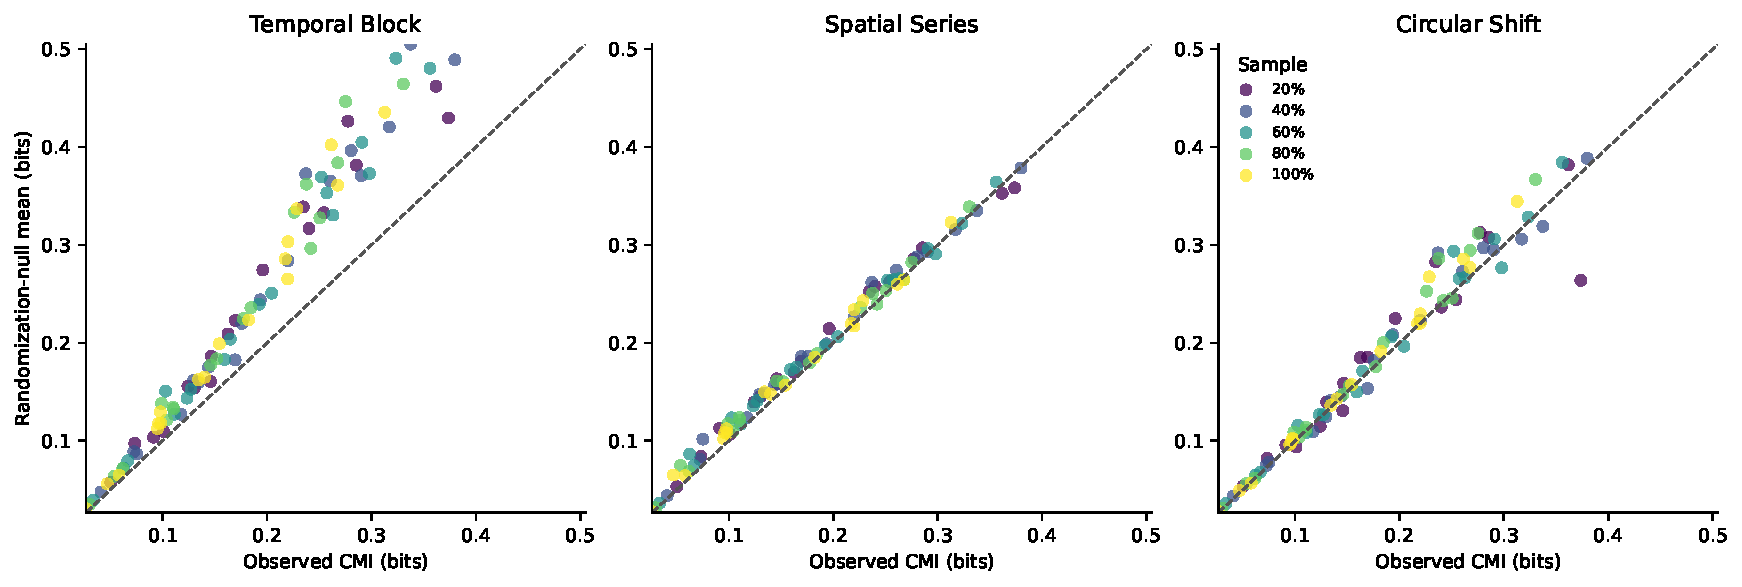
\includegraphics[width=\linewidth]{figures/e16/e16_s16_6_observed_vs_null.pdf}
\end{adjustwidth}
\caption{270项城市--空间--时间--样本--设计比较中的观测Miller--Madow CMI与随机化
参考均值。虚线表示相等；非零参考中心是允许的，且不等于总体CMI。}
\label{fig:e16_observed_null}
\end{figure}

对图~\ref{fig:e16_observed_null} 而言，对角线上方的点仅表示观测统计量大于参考
均值，这一视觉条件本身不是拒绝准则。推断结论由上尾概率和预设 FDR 校正共同决定。

这些结果把主要1~km分析扩展到多种聚合尺度，但不改变其解释：不同尺度均出现正的
DELB下降点估计，预设多尺度校准在多重比较修正后未识别出自行车特异信息。

\subsection{实际预测与 Predictability Gap}
\label{subsec:results_prediction}

预测分析检验特定拟合模型能否在未见观测中利用增强状态，因此被有意置于 DELB 估计
之后。理论界描述给定信息集下可达到的最小 MSE；图~\ref{fig:mse_improvement}
则报告具体有限样本估计器实际获得的变化。正柱表示自行车增强模型更优，但本身不能
识别信息来源。

固定的 2022 年 7--12 月测试集包含 75,992 个网格--日。在 12 个城市--模型
组合中，加入自行车状态后有 6 个组合的 MSE 点估计下降；其中
\PositiveMatchedModels{} 个组合通过调整后的正改善筛查：纽约的状态均值模型和
梯度提升模型，以及温哥华的状态均值模型。其余设定不变或变差。

\begin{figure}[H]
\centering
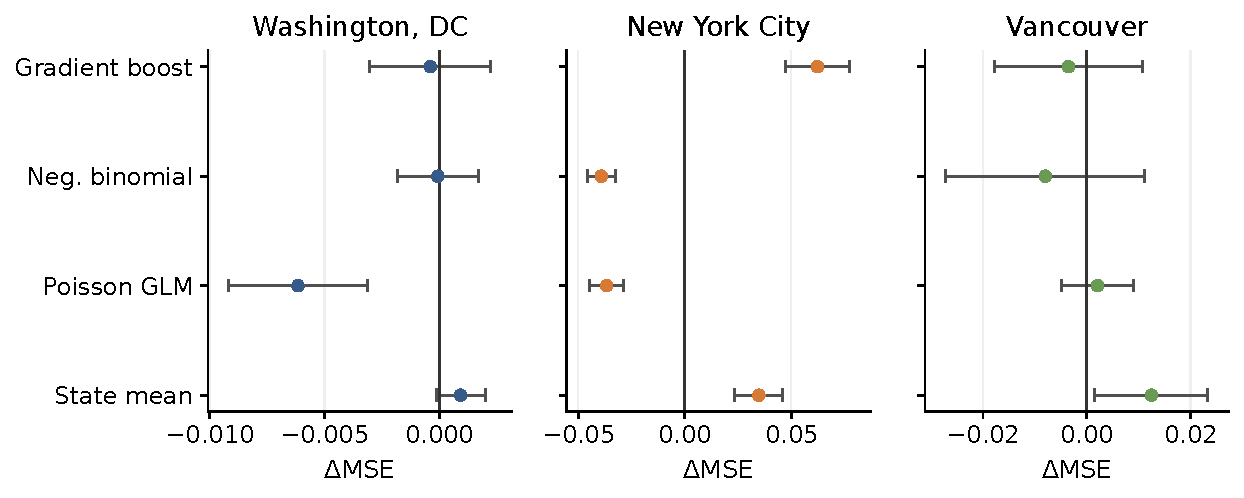
\includegraphics[width=\textwidth]{figures/e11/e06_mse_improvement.pdf}
\caption{加入滞后自行车状态后的留出整数 MSE 变化。正值有利于自行车增强设定；
比较在同一城市和模型族内配对进行。}
\label{fig:mse_improvement}
\end{figure}


\begin{table}[!htbp]
\caption{Matched held-out integer-prediction MSE, DELB, and Predictability Gap results for July--December 2022. The paired DELB column reports the baseline and bicycle-augmented lower bounds as \(L^0/L^B\). Positive \(\Delta\mathrm{MSE}\) denotes lower error after adding bicycle information. Gap narrowing is \(\Delta G=\Delta\mathrm{MSE}-\Delta L\): a positive value indicates that the model moved closer to the lower bound, whereas a negative value indicates that the estimated lower bound decreased more than the model MSE. Differences were calculated from unrounded values and then rounded for display.}
\label{tab:prediction_gap_results}
\begin{adjustwidth}{-\extralength}{0cm}
\raggedleft
\begin{tabular*}{\linewidth}{@{\extracolsep{\fill}}llrrrrrr@{}}
\toprule
\textbf{City} & \textbf{Model} & \(\boldsymbol{\mathrm{MSE}^0}\) &
\(\boldsymbol{\mathrm{MSE}^B}\) & \(\boldsymbol{L^0/L^B}\) &
\(\boldsymbol{\Delta\mathrm{MSE}}\) &
\(\boldsymbol{\Delta L}\) & \textbf{Gap narrowing}\\
\midrule
Washington, DC & State mean & \rev{0.5002} & \rev{0.4993} & 0.107/0.092 & \rev{0.0009} & 0.015 & -0.014\\
Washington, DC & Poisson GLM & \rev{0.4933} & \rev{0.4994} & 0.107/0.092 & \rev{-0.0062} & 0.015 & -0.021\\
Washington, DC & Negative-binomial GLM & \rev{0.4931} & \rev{0.4932} & 0.107/0.092 & \rev{-0.0001} & 0.015 & -0.015\\
Washington, DC & Poisson gradient boosting & \rev{0.4952} & \rev{0.4956} & 0.107/0.092 & \rev{-0.0004} & 0.015 & -0.016\\
New York City & State mean & \rev{2.0893} & \rev{2.0545} & 0.263/0.230 & \rev{0.0348} & 0.034 & 0.001\\
New York City & Poisson GLM & \rev{1.9043} & \rev{1.9410} & 0.263/0.230 & \rev{-0.0367} & 0.034 & -0.070\\
New York City & Negative-binomial GLM & \rev{1.9073} & \rev{1.9465} & 0.263/0.230 & \rev{-0.0392} & 0.034 & -0.073\\
New York City & Poisson gradient boosting & \rev{1.9010} & \rev{1.8388} & 0.263/0.230 & \rev{0.0623} & 0.034 & 0.029\\
Vancouver & State mean & \rev{1.6632} & \rev{1.6507} & 0.259/0.208 & \rev{0.0125} & 0.051 & -0.038\\
Vancouver & Poisson GLM & \rev{1.6287} & \rev{1.6266} & 0.259/0.208 & \rev{0.0021} & 0.051 & -0.049\\
Vancouver & Negative-binomial GLM & \rev{1.6138} & \rev{1.6218} & 0.259/0.208 & \rev{-0.0080} & 0.051 & -0.059\\
Vancouver & Poisson gradient boosting & \rev{1.6654} & \rev{1.6690} & 0.259/0.208 & \rev{-0.0035} & 0.051 & -0.054\\
\bottomrule
\end{tabular*}
\end{adjustwidth}
\end{table}


全部测试 MSE 均高于其匹配的精确 DELB。只有纽约状态均值模型
（\(\Delta G=0.001\)）和纽约梯度提升模型（\(\Delta G=0.029\)）缩小了
Predictability Gap；其余组合的 \(\Delta G\) 均为负。因此，更低的估计底线
与有利的实际误差响应在经验上是两个不同对象。

\begin{figure}[H]
\centering
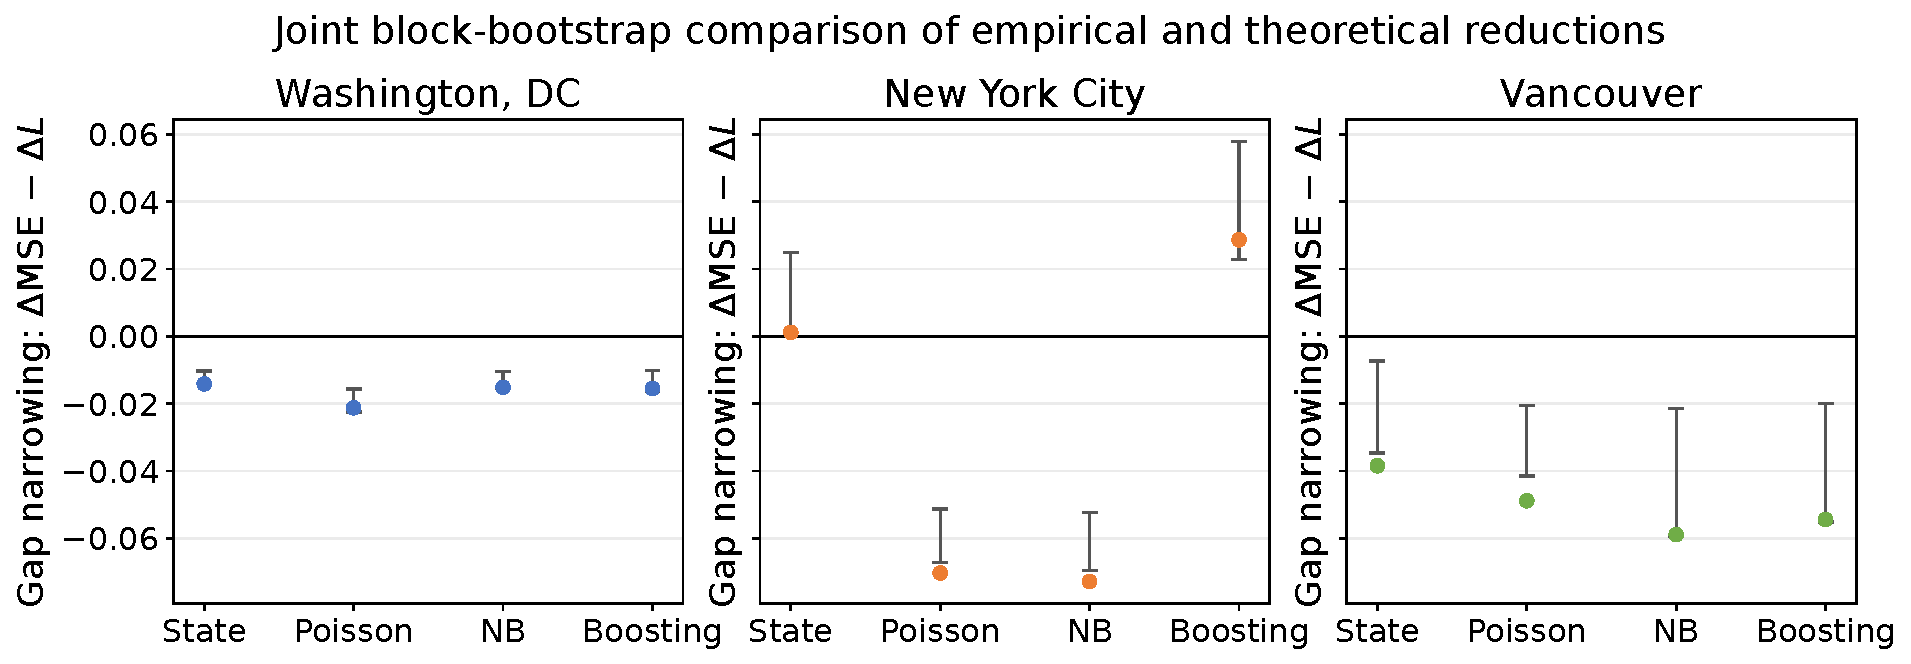
\includegraphics[width=\textwidth]{figures/e11/e07_gap_narrowing.pdf}
\caption{加入自行车状态后的 Predictability Gap 缩小量。正值表示经验 MSE 的
下降超过估计 DELB 的下降；负值表示未利用的信息空间变大。}
\label{fig:gap_narrowing}
\end{figure}

综合解释是：新增状态变量产生了估计预测机会，但只有部分模型--城市组合把这种机会
转化为留出精度。负的 gap 变化不违反 DELB；它表示实际误差下降不足以抵消估计底线
的变化。

\subsection{次要与稳健性结果}

\subsubsection{Fano 分类损失对照}
\label{subsec:results_fano}

Fano 是损失函数特异的交叉检查，而不是计数 MSE 底线的第二个估计。Oracle 面板在
总体分布已知时核查不等式；经验面板则检验透明的众数分类器是否高于测试前估计的分类
底线。因此，较低的底线与较低的分类器错误率仍是两个不同量。

全部 \FanoOracleRows{} 个总体 oracle 比较均满足真实 Fano 不等式，所有留出
众数分类器误差也均高于其测试前估计底线；点估计违反数为
\FanoEstimatedViolations{}。在全部 \FanoTotalContrasts{} 个城市--目标比较中，
加入自行车状态均使 Miller--Madow Fano 底线下降，降幅为
\FanoFloorReductionMin{}--\FanoFloorReductionMax{}。但随着测试期未见状态
增加，众数分类器误差在 \FanoNegativeTestContrasts{}/\FanoTotalContrasts{}
个比较中上升。

\begin{table}[!htbp]
\caption{\rev{Miller--Madow Fano floors and held-out statewise modal-classifier errors. The interval refers to the baseline-minus-bicycle floor reduction. The final column gives baseline/bicycle-aware counts of test observations assigned through the pretest global-mode fallback because their states were unseen before testing.}}
\label{tab:e14_fano_results}
\centering
\small
\setlength{\tabcolsep}{2.5pt}
\begin{tabular*}{\textwidth}{@{\extracolsep{\fill}}llccccc@{}}
\toprule
\textbf{City} & \textbf{Target} & \textbf{Base floor} & \textbf{Bike floor} & \textbf{Reduction [95\% CI]} & \textbf{Test error} & \shortstack{\textbf{Unseen test}\\\textbf{observations}}\\
\midrule
Washington, DC & Binary occurrence & 0.126 & 0.115 & 0.010 [0.010, 0.011] & 0.200/0.205 & 865/2,071\\
Washington, DC & Three-level count & 0.133 & 0.122 & 0.012 [0.011, 0.013] & 0.232/0.235 & 865/2,071\\
New York City & Binary occurrence & 0.150 & 0.124 & 0.027 [0.024, 0.029] & 0.358/0.364 & 2,058/4,408\\
New York City & Three-level count & 0.181 & 0.151 & 0.030 [0.027, 0.033] & 0.445/0.450 & 2,058/4,408\\
Vancouver & Binary occurrence & 0.200 & 0.175 & 0.025 [0.022, 0.028] & 0.326/0.335 & 234/812\\
Vancouver & Three-level count & 0.261 & 0.224 & 0.038 [0.034, 0.041] & 0.393/0.401 & 234/812\\
\bottomrule
\end{tabular*}
\end{table}


\begin{figure}[H]
\begin{adjustwidth}{-\extralength}{0cm}
\centering
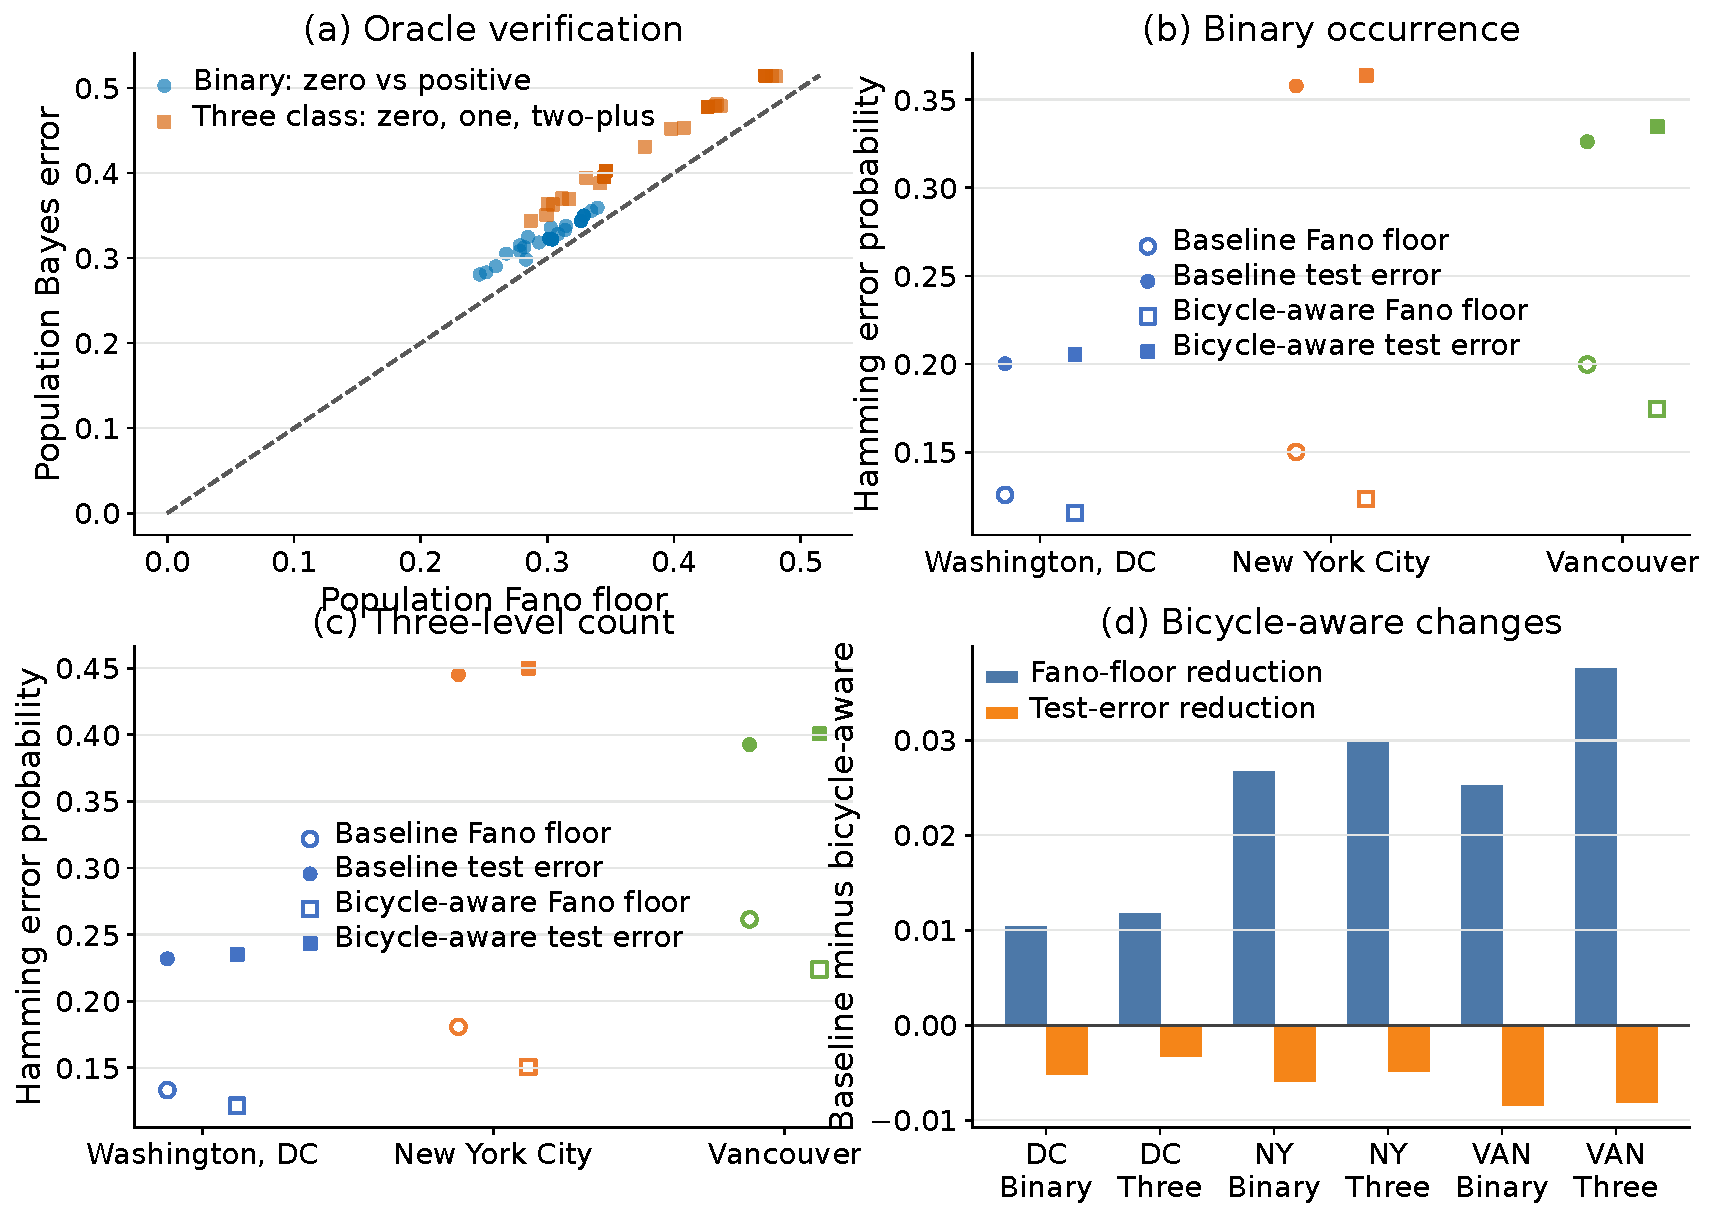
\includegraphics[width=\linewidth]{figures/s7/e14_fano_main.pdf}
\end{adjustwidth}
\caption{Fano 分类损失对照。Oracle 面板比较真实 Bayes 误差与真实 Fano 底线；
经验面板比较测试前估计底线与留出众数分类器误差。}
\label{fig:e14_fano}
\end{figure}

这种方向差异不是 Fano 违反。增加信息可以降低总体底线，同时使稀疏有限样本
分类器变差。Fano 与 DELB 的降幅使用不同目标和损失，数值不能直接比较。

\subsubsection{犯罪类型异质性}
\label{subsec:results_crime_types}

该分析检验描述性 DELB 模式是否集中于某个统一犯罪类别。由于主要随机化校准没有在
每个类别内重复完成，因此该结果属于探索性分析；完整表图见补充材料 S4。

全部 \PositiveCrimeTypeTheory{} 个城市--类别汇总 CMI 点估计均为正。每个城市
均以财产盗窃的 \(\Delta L\) 最大：华盛顿特区 0.009、纽约 0.045、温哥华
0.060。36 个匹配的城市--类别--模型比较中，只有 4 个通过调整后的正预测改善
筛查，且全部位于纽约；只有财产盗窃的梯度提升模型同时缩小 gap。由于零分布校准
针对汇总犯罪完成，这些分类结果仍属探索性分析。

\subsubsection{替代设定与滚动起点}
\label{subsec:results_robustness}

替代理论设定检验点估计符号对不同操作定义是否稳健；滚动起点检验实际模型表现的时间
重复性。两者都不能取代随机化归因检验。

三个城市的 16 个预设理论替代设定中，plugin、Miller--Madow 和一致的
observed-support Jeffreys--Dirichlet \(\Delta L\) 均为正。符号在空间和
时间聚合、状态映射、估计量、滞后期及流量定义之间保持一致。由于目标
与 MSE 单位改变，不同网格尺度或周目标的数值并不是可直接比较的效应量。

滚动预测仍依赖模型和城市。纽约梯度提升在全部 12 个月度起点均改善
（平均 \(\Delta\mathrm{MSE}=0.076\)），其状态均值模型在 11 个起点改善
（平均 0.030）。华盛顿特区和温哥华的状态均值模型均在 8 个起点改善，
平均增益分别为 0.001 和 0.006。多数 GLM 的平均变化为负。完整滚动起点表图见
补充材料 S5。
